\section{Steps}

\subsection{Einbinden von Nuitrack}
Nuitrack kann unter folgendem Link für alle Platformen runtergeladen werden: \href{https://github.com/3DiVi/nuitrack-sdk/blob/master/doc/Install.md} .

\subsubsection{Import Nuitrack Wrapper in Unity}
Unter folgendem git repo kann das Nuitrack Plugin runtergeladen werden: \href{https://github.com/3DiVi/nuitrack-sdk/blob/master/Unity3D/NuitrackSDK.unitypackage} . Da dieses Plugin für verschiede Sensoren, also Kameras konfiguriert wurde, muss dann noch der Sensor spezifiziert werden. In meinem Projekt ist dies die IntelRealsense D435.


\subsubsection{Skeleton Tracking mit NuitrackSDK}
Das Tutorial von Nuitrack ist meine Ausgangslage um eine Person zu tracken. Der Link führt zu diesem Tutorial: \href{https://github.com/3DiVi/nuitrack-sdk/blob/master/doc/Unity_Face_Tracking.md} .

\subsection{Virtuelle Szene in Unity}
In Unity baue ich die Szene so auf, dass die Render-Kamera in positiver z-Achse ausgerichtet ist. Anfangsposition der Render-Kamera ist (0, 0.2, -1.5). Den Screen welcher dann entzerrt werden soll, setze ich auf den Nullpunkt. Also genauer die Mitte vom Screen hat die Position (0, 0, 0).
Die Eckpunkte vom Screen haben die folgenden Positionen: 
P0(-0.8, -0.45)
P1( 0.8, -0.45)
P2( 0.8,  0.45)
P3(-0.8,  0.45)
Der Screen hat die Grösse 1600 x 900 mm. Dieser wird als schmaler Kubus dargestellt und transparent leicht grau eingefärbt, damit ich dann erkannen kann ob mein Rendern und Entzerren richtig funktioniert.
Die Main-Kamera setze ich als Referenz auf die Position der Render-Kamera. Dies damit ich eine Ansicht in der Szene bekomme. Die Main-Kamera zeigt dann die Szene und für den Output vom entzerrten Screen benötige ich das gerenderte Bildmaterial der Renderkamera. 
Gut möglich, dass man dies auch mit weniger Kameras darstellen kann.

\subsubsection{Render Kamera zeigt Position vom Betrachter}
Die Render-Kamera wird als Referenz auf den obersten Knochen vom Skelett gemappt. Dieser oberste Knochen entspricht dem Kopf, genauer der Stirn.
Damit wird dann auch die Main-Kamera, welche die Render-Kamera referenziert auf den Kopf gemappt.

\subsubsection{Render Kamera zeigt RenderTexture}
Die Render-Kamera wird nun stets auf den Mittelpunkt vom Screen gerichtet. Der Output der Render-Kamera erzeugt dann eine RenderTexture der Grösse 750 x 750 Pixel. Je grösser die Anzahl Pixel, desto besser wird dann die Qualität vom Endbild.

\subsection{Matrix Shader}
Im Netz habe ich einen Rotations Shader gefunden und versucht diesen so anzupassen, dass die Entzerrung gelingt. Leider ohne Erfolg. Das Probelm bei diesem Shader funktioniert das Scaling und das Shearing, nicht aber die Translation. Zudem wüsste ich nicht, wie ich mit dieser Rotationsmatrix das Polygon selektieren sollte.
Als Einstieg in die Unity Shader hat es trotzdem etwas geholfen, mehr aber auch nicht.

\subsection{Pixel Shader}
Damit ich diese Entzerrung vom Polygon machen kann, benötige ich einen Pixel-Shader. Oder einen Shader welcher die Maintexture ändert.
So habe ich nun einen Shader welche als Parameter die Maintextur als Eingabewert hat. Im Script wird dann in der Update Funktion für jedes Pixel der Farbwert gesetzt und am Ende die Textur dem Shader übergeben.

\subsection{Entzerrung vom Polygon}
\subsubsection{Homographie}
Zuerst habe ich versucht die Entzerrung mit einer Homographie Matrix zu erreichen. Leider hat dies nur geklappt für die Ansicht ohne seitliche Verschiebung, also mit einem x-Wert von Null. Sobald ich etwas abweiche von dieser zentralen Position, zeigt sich ein Shearing im Output Bild, welches sich auch noch anders verhält, je nachdem ich in positiver x-Achse gehe oder in negativer x-Achse. 
Ich habe da länger darüber nachgedacht, meine Homographie Matrix mehrmals geprüft, fand aber nicht heraus was das Problem war. Komisch ja auch, dass es in zentraler Position den Richtigen Output gab, bei seitlicher Verschiebung sich dann aber ein Shearing zeigt, welches mit grösserer Abweichung nach links oder rechts dann auch noch grösser wurde.
Somit brauche ich einen anderen Ansatz um die Entzerrung zu lösen.

\subsubsection{OpenCV}
OpenCV hat bereits Methoden, welche diese Entzerrung vornehmen. Das Plugin von OpenCV findet sich unter: \href{https://github.com/EnoxSoftware/OpenCVForUnity/tree/master/Assets/OpenCVForUnity} .
Die grösste Schwierigkeit ist bei OpenCV, dass Unity einen anderen Aufbau der Matrizen hat und dass OpenCV keine Textures kennt. 
Die grösste Schwierigkeit war dann zu merken, dass die Pixelwerte der Textures in OpenCV nicht einfach so auf der CPU verfügbar sind. Diese werden auf der GPU gespeichert und mössen dann exklusiv abgefragt werden.
Die Funktionen von OpenCV funktionieren tadellos. Damit die Entzerrung gelingt, gehe ich vom Zielbild aus und berechne die Perspektivische Matrix rückwärts vom Zielbild zum Inputbild, was dann dem Inversen der Perspektivischen Matrix entspricht. 
Nun wird diese Matrix auf jedes Pixel des Zielbildes angewendet und so den Farbwert an der entsprechenden Stelle im Inputbild geholt. 
Da diese Operation mit der Anzahl Pixel steigt, habe ich hier ein Format vom Zielbild 800 x 450 Pixel gewählt.

\subsection{Berechnung der Polygon Eckpunkte}
\subsubsection{Kameramodell}
Ich habe versucht mittels Kameramodell die Transformationsmatrix für die Eckpunkte vom Screen zu berechnen. Dazu braucht man den Viewport, die intrinsiche (Projektionsmatrix) und die extrinsische Kameramatrix (Viewmatrix). Da sich der Screen nicht verschiebt, braucht es die Modellmatrix nicht.
 
\subsubsection{Projektion der Eckpunkte auf der Zielebene}
Mein Ansatz den ich umgesetzt habe funktioniert wie folgt: 
Unity hat eine Funktion welche mir die Eckpunkte von der Clipping Ebene entsprechend dem z Wert herausscheibt. Ich wähle diese Ebene durch den Nullpunkt, auf welchen sich die Render-Kamera immer richtet. 
Nun projeziere ich die Eckpunkte vom Screen in der Verlängerung von der Render-Kamera durch die Eckpunkte. Die Schnittpunkte mit der Ebene müssen nun nur noch relativ zu den Ecken der Clipping Ebene berechnet werden. 

\subsection{Tabular}

\begin{tabular}[h]{l|l|l}
  \centering
	Measure & Data & Unit \\ \hline
	1      & 2	  & 3  \\
	4      & 5	  & 6
\end{tabular}

% Example for a Table in BFH-Style with a simple Design
\begin{table}[ht]
   \centering
   \begin{bfhTabular}{lll}
      Stadtteil & Anzahl Personen & Ausländische
      Bevölkerung\\\hline
      Innere Stadt & \num{3748} & \SI{17.9}{\percent}\\\hline
      Länggasse-Felsenau & \num{17976} & \SI{17.1}{\percent}\\\hline
      Mattenhof-Weissenbühl & \num{26895} & \SI{22.4}{\percent}\\\hline
      Kirchenfeld-Schlosshalde & \num{23384} & \SI{13.4}{\percent}\\\hline
      Breitenrain-Lorraine & \num{24082} & \SI{19.4}{\percent}
   \end{bfhTabular}
   \caption{Anzahl Personen, ausländischer Bevölkerungsanteil und Arbeitslosenquote pro
	Stadtteil Ende 2005 (Statistikdienste der Stadt Bern, 2006)}
   \label{tab:tab1}
\end{table}

\begin{table}[ht]
   \centering
   \colorlet{BFH-table}{BFH-MediumBlue!10}
   \colorlet{BFH-tablehead}{BFH-MediumBlue!50}
   \begin{bfhTabular}{lll}
      Stadtteil & Anzahl Personen & Ausländische
      Bevölkerung\\\hline
      Innere Stadt & \num{3748} & \SI{17.9}{\percent}\\\hline
      Länggasse-Felsenau & \num{17976} & \SI{17.1}{\percent}\\\hline
      Mattenhof-Weissenbühl & \num{26895} & \SI{22.4}{\percent}\\\hline
      Kirchenfeld-Schlosshalde & \num{23384} & \SI{13.4}{\percent}\\\hline
      Breitenrain-Lorraine & \num{24082} & \SI{19.4}{\percent}
   \end{bfhTabular}
   \caption{Anzahl Personen, ausländischer Bevölkerungsanteil und Arbeitslosenquote pro
	Stadtteil Ende 2005 (Statistikdienste der Stadt Bern, 2006)}
   \label{tab:tab2}
\end{table}

\begin{table}[ht]
   \centering
   \colorlet{BFH-table}{BFH-MediumRed!10}
   \colorlet{BFH-tablehead}{BFH-MediumRed!50}
   \begin{bfhTabular}{lll}
      Stadtteil & Anzahl Personen & Ausländische
      Bevölkerung\\\hline
      Innere Stadt & \num{3748} & \SI{17.9}{\percent}\\\hline
      Länggasse-Felsenau & \num{17976} & \SI{17.1}{\percent}\\\hline
      Mattenhof-Weissenbühl & \num{26895} & \SI{22.4}{\percent}\\\hline
      Kirchenfeld-Schlosshalde & \num{23384} & \SI{13.4}{\percent}\\\hline
      Breitenrain-Lorraine & \num{24082} & \SI{19.4}{\percent}
   \end{bfhTabular}
   \caption{Anzahl Personen, ausländischer Bevölkerungsanteil und Arbeitslosenquote pro
	Stadtteil Ende 2005 (Statistikdienste der Stadt Bern, 2006)}
   \label{tab:tab3}
\end{table}


\begin{description}
\item[More about Tables] Further information about tables : \url{https://www.latex-tutorial.com/tutorials/tables/}
\item[Long Tables] Further information about long tables : \url{https://www.overleaf.com/learn/latex/tables}
\end{description}


\begin{longtable}{|l|l|l|}
\caption{A sample long table} \label{tab:long} \\


\hline \multicolumn{1}{|c|}{\textbf{First column}} & \multicolumn{1}{c|}{\textbf{Second column}} & \multicolumn{1}{c|}{\textbf{Third column}} \\ \hline 
\endfirsthead

\multicolumn{3}{c}%
{{\tablename\ \thetable{}: \hfill $...$~continued from previous page}} \\
\hline \multicolumn{1}{|c|}{\textbf{First column}} & \multicolumn{1}{c|}{\textbf{Second column}} & \multicolumn{1}{c|}{\textbf{Third column}} \\ \hline 
\endhead

\hline \multicolumn{3}{|r|}{{Continued on next page$...$}} \\ \hline
\endfoot

\hline \hline
\endlastfoot
\centering

One & abcdef ghjijklmn & 123.456778 \\
One & abcdef ghjijklmn & 123.456778 \\
One & abcdef ghjijklmn & 123.456778 \\
One & abcdef ghjijklmn & 123.456778 \\
One & abcdef ghjijklmn & 123.456778 \\
One & abcdef ghjijklmn & 123.456778 \\
One & abcdef ghjijklmn & 123.456778 \\
One & abcdef ghjijklmn & 123.456778 \\
One & abcdef ghjijklmn & 123.456778 \\
One & abcdef ghjijklmn & 123.456778 \\
One & abcdef ghjijklmn & 123.456778 \\
One & abcdef ghjijklmn & 123.456778 \\
One & abcdef ghjijklmn & 123.456778 \\
One & abcdef ghjijklmn & 123.456778 \\
One & abcdef ghjijklmn & 123.456778 \\
One & abcdef ghjijklmn & 123.456778 \\
One & abcdef ghjijklmn & 123.456778 \\
One & abcdef ghjijklmn & 123.456778 \\
One & abcdef ghjijklmn & 123.456778 \\
One & abcdef ghjijklmn & 123.456778 \\
One & abcdef ghjijklmn & 123.456778 \\
One & abcdef ghjijklmn & 123.456778 \\
One & abcdef ghjijklmn & 123.456778 \\
One & abcdef ghjijklmn & 123.456778 \\
One & abcdef ghjijklmn & 123.456778 \\
One & abcdef ghjijklmn & 123.456778 \\
One & abcdef ghjijklmn & 123.456778 \\
One & abcdef ghjijklmn & 123.456778 \\
One & abcdef ghjijklmn & 123.456778 \\
One & abcdef ghjijklmn & 123.456778 \\
One & abcdef ghjijklmn & 123.456778 \\
One & abcdef ghjijklmn & 123.456778 \\
One & abcdef ghjijklmn & 123.456778 \\
One & abcdef ghjijklmn & 123.456778 \\
One & abcdef ghjijklmn & 123.456778 \\
One & abcdef ghjijklmn & 123.456778 \\
One & abcdef ghjijklmn & 123.456778 \\
One & abcdef ghjijklmn & 123.456778 \\
One & abcdef ghjijklmn & 123.456778 \\
One & abcdef ghjijklmn & 123.456778 \\
One & abcdef ghjijklmn & 123.456778 \\
One & abcdef ghjijklmn & 123.456778 \\
One & abcdef ghjijklmn & 123.456778 \\
One & abcdef ghjijklmn & 123.456778 \\
One & abcdef ghjijklmn & 123.456778 \\
One & abcdef ghjijklmn & 123.456778 \\
One & abcdef ghjijklmn & 123.456778 \\
One & abcdef ghjijklmn & 123.456778 \\
One & abcdef ghjijklmn & 123.456778 \\
One & abcdef ghjijklmn & 123.456778 \\
One & abcdef ghjijklmn & 123.456778 \\
One & abcdef ghjijklmn & 123.456778 \\
One & abcdef ghjijklmn & 123.456778 \\
One & abcdef ghjijklmn & 123.456778 \\
One & abcdef ghjijklmn & 123.456778 \\
One & abcdef ghjijklmn & 123.456778 \\
One & abcdef ghjijklmn & 123.456778 \\
One & abcdef ghjijklmn & 123.456778 \\
One & abcdef ghjijklmn & 123.456778 \\
One & abcdef ghjijklmn & 123.456778 \\
One & abcdef ghjijklmn & 123.456778 \\
One & abcdef ghjijklmn & 123.456778 \\
One & abcdef ghjijklmn & 123.456778 \\
One & abcdef ghjijklmn & 123.456778 \\
One & abcdef ghjijklmn & 123.456778 \\
One & abcdef ghjijklmn & 123.456778 \\
One & abcdef ghjijklmn & 123.456778 \\
One & abcdef ghjijklmn & 123.456778 \\
One & abcdef ghjijklmn & 123.456778 \\
One & abcdef ghjijklmn & 123.456778 \\
One & abcdef ghjijklmn & 123.456778 \\
One & abcdef ghjijklmn & 123.456778 \\
One & abcdef ghjijklmn & 123.456778 \\
One & abcdef ghjijklmn & 123.456778 \\
One & abcdef ghjijklmn & 123.456778 \\
\end{longtable}
 

\subsection{Math}
%% Mathematical equations
\begin{align}
\left(\begin{array}{r}
\dot{x_{1}} \\                                              
\dot{x_{2}} \\ 
\dot{x_{3}} \\                                 
\end{array}\right) =
\left[\begin{array}{rrr}
0 & 1 & 0 \\                                              
0 & -\frac{b_{f}}{J} & \frac{K_{m}}{J} \\
0 & -\frac{K_{g}}{L} & \frac{R}{L} \\                                      
\end{array}\right]
\left(\begin{array}{r}
x_{1} \\                                              
x_{2} \\ 
x_{3} \\                                 
\end{array}\right) +
\left[\begin{array}{rr}
0 & 0 \\                                              
-\frac{1}{J} & 0 \\ 
0 & \frac{1}{L} \\                                 
\end{array}\right]
\left(\begin{array}{r}
t_{L} \\                                              
v_{a} \\                                 
\end{array}\right)
\end{align}

\subsection{Include pictures}

\begin{figure}[H]
  \centering
  
\includegraphics[width=.8\textwidth]{placeholder}
  \caption{Some meaningful caption}
  \label{fig:placeholder:1}
\end{figure}


\begin{figure}[h!]
  \centering
  \begin{minipage}{.4\textwidth}
  	\centering
	
\includegraphics[width=\textwidth]{placeholder}
	\caption{PLACEHOLDER}
	\label{fig:placeholder:2}
  \end{minipage}
  \hspace{1em}
  \begin{minipage}{.4\textwidth}
	\centering
	
\includegraphics[width=\textwidth]{placeholder}
	\caption{PLACEHOLDER}
	\label{fig:placeholder:3}
  \end{minipage}%
\end{figure}


%% Source code is stored in the listings folder and will be included from there using its relative path.
\subsection{Code Example}

{
  \thicklines
% \thinlines
\lstinputlisting[style=bfh-c,language=C,caption={My very first C program.},label={lst:hello}]{listings/expl_hello.c}
}
I developed this very nice application writing "Hello World" to my terminal.
The implementation is shown in listing~\ref{lst:hello}.


%% Examples holding dummy content
\subsection{Draw boxes}
\begin{bfhBox}[BFH-DarkPurple]{Purple}
	Note\\
\end{bfhBox}

\blindtext[1]

\begin{bfhBox}[BFH-MediumBlue]{Blue}
	Note\\
\end{bfhBox}

\blindtext[1]

\begin{bfhBox}[BFH-DarkRed]{Red}
	Note\\
\end{bfhBox}

\blindtext[2]

\begin{bfhAlertBox}
  An alert box.
\end{bfhAlertBox}

\begin{bfhWarnBox}
  A warning box.
\end{bfhWarnBox}

\begin{bfhNoteBox}
  A note box.
\end{bfhNoteBox}

\begin{bfhRecycleBox}
  A recycle box.
\end{bfhRecycleBox}


\begin{bfhBox}{No color set}
	Some BFH box without color option set. Using default.\\
\end{bfhBox}


\blindtext[3]


\subsection{Some Item-list}
Sometimes you explain this and that using a bullet points.
This can be done in \LaTeX\ using an item list in a item environment.

\begin{itemize}
\item My first item
\item The second
\item $\cdots$
\item $\cdots$
\end{itemize}

It is also possible to nest such environment and/or enumerate.
\begin{itemize}
\item My first item
\begin{enumerate}
\item My first enumerated item
\item The second
\item $\cdots$
\end{enumerate}
\item The second
\begin{enumerate}
\item An other enumerated item
\item $\cdots$
\item $\cdots$
\end{enumerate}
\end{itemize}


\subsection{Multi column environment}
Split a part of a document in multiple columns is not so easy with WYSIWYG tools.
Whit multicols \LaTeX\ package$\cdots$ well you may know.

\begin{multicols}{3}
\begin{itemize}
\item My first item
\item The second
\item $\cdots$
\item $\cdots$
\end{itemize}
\begin{itemize}
\item My first item
\item The second
\item $\cdots$
\item $\cdots$
\end{itemize}
\begin{itemize}
\item My first item
\item The second
\item $\cdots$
\item $\cdots$
\end{itemize}
\end{multicols}


\blindtext[1]

\begin{multicols}{2}
  \blindtext[1]
\end{multicols}

\begin{multicols}{3}
  \blindtext[1]
\end{multicols}

\begin{multicols}{2}
  \blindtext[1]
\end{multicols}


\begin{multicols}{3}
\begin{itemize}
\item My first item
\item The second
\item $\cdots$
\item $\cdots$
\end{itemize}
\blindtext[1]
\columnbreak
\begin{itemize}
\item My first item
\item The second
\item $\cdots$
\item $\cdots$
\end{itemize}
\end{multicols}

%% forced page break
\newpage

\subsection{Use Figures}

\begin{figure}[h!]
  \centering
  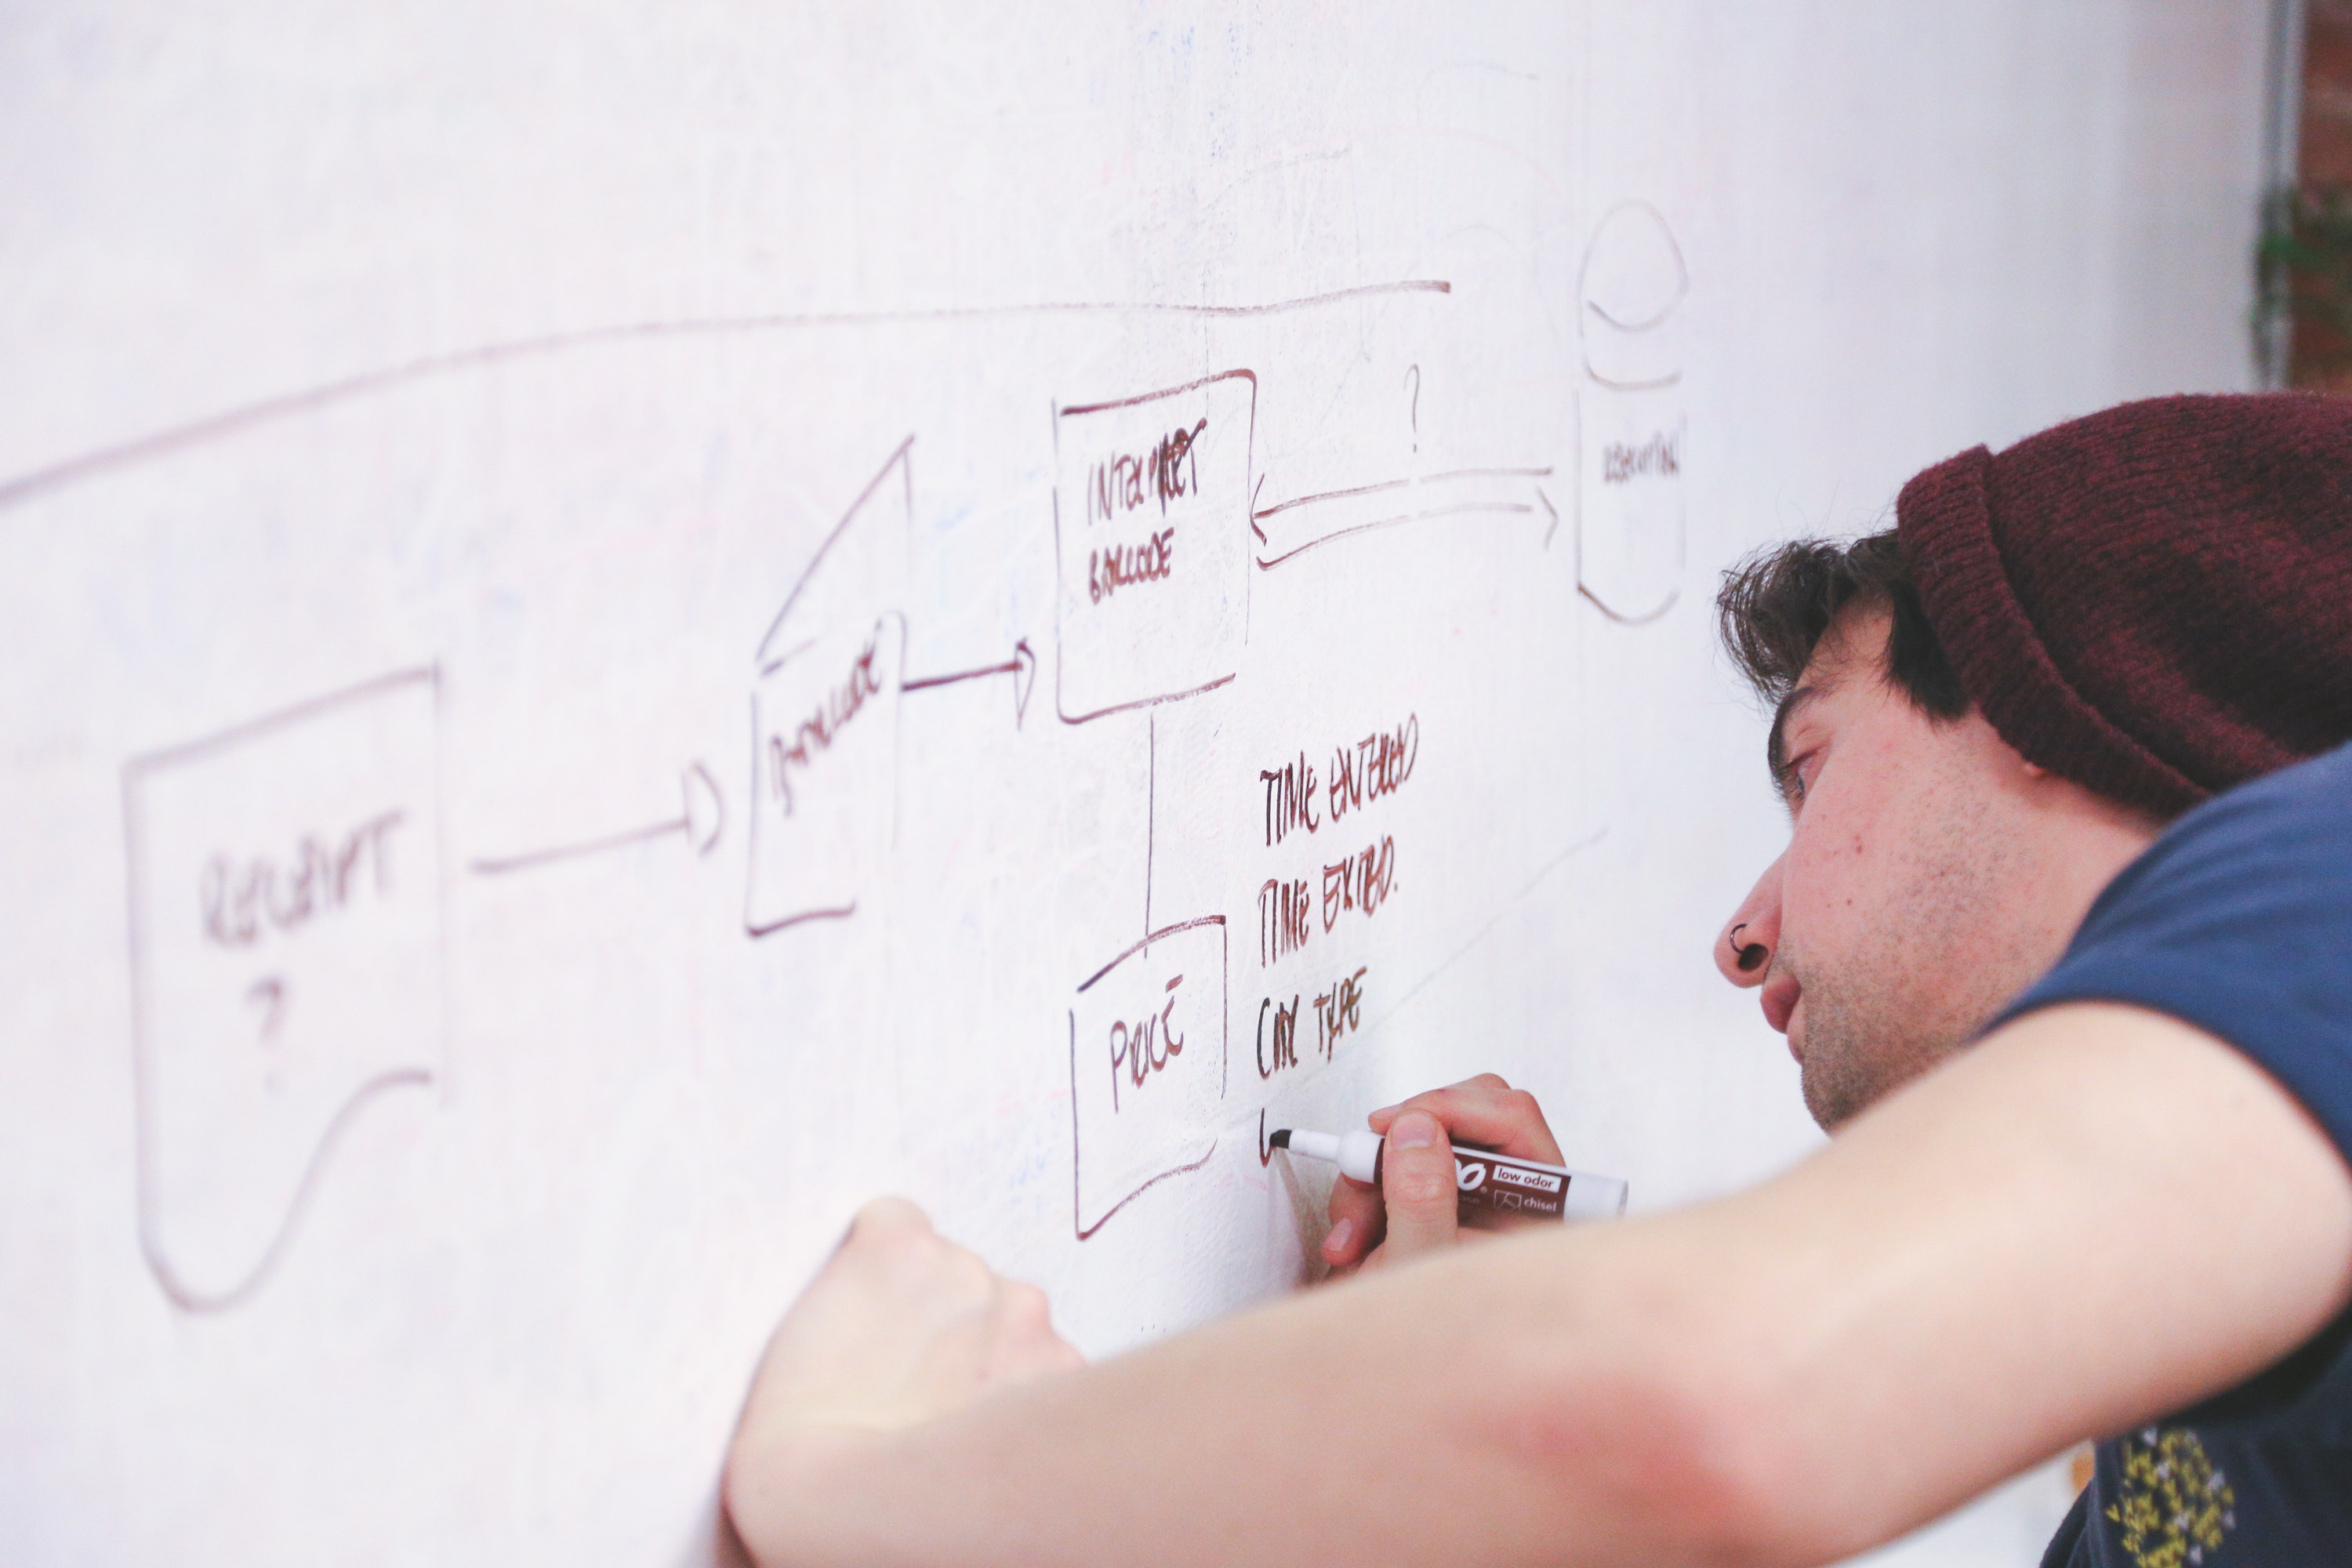
\includegraphics[width=.8\textwidth]{bg-masthead}
  \caption{An example of including a PDF figure.}
  \label{fig:expl_master}
\end{figure}

\begin{figure}[h!]
  \centering
  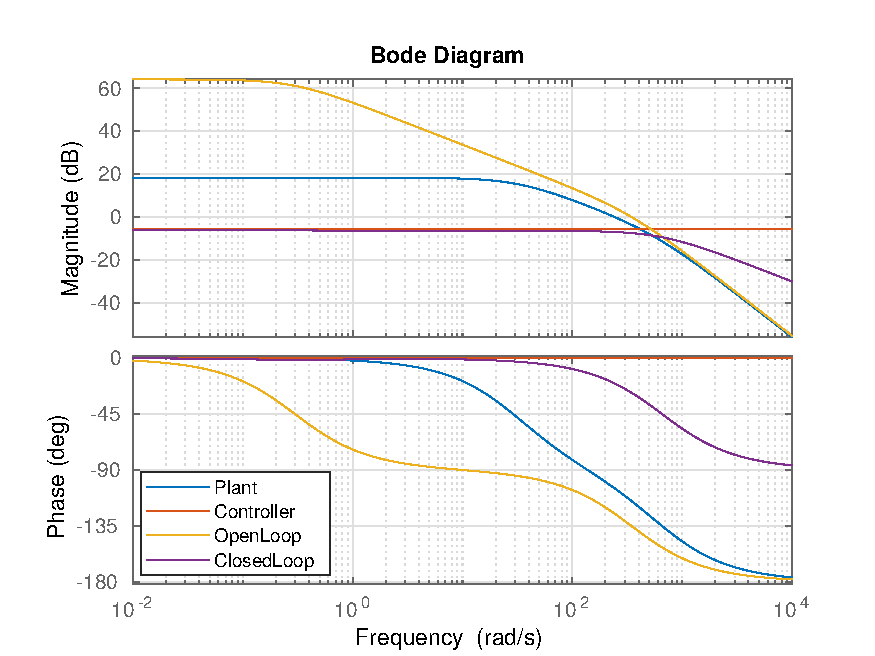
\includegraphics[width=.8\textwidth]{expl_bode}
  \caption{An example of including a PDF figure.}
  \label{fig:expl_bode}
\end{figure}
\clearpage

\subsubsection{Use Subfigures}
These subfigures requires the package \texttt{subcaption}.

\begin{figure}[h!]
     \centering
     \begin{subfigure}[b]{0.3\textwidth}
         \centering
         
\includegraphics[width=\textwidth]{placeholder}
         \caption{$y=x$}
         \label{fig:y equals x}
     \end{subfigure}
     \hfill
     \begin{subfigure}[b]{0.3\textwidth}
         \centering
         
\includegraphics[width=\textwidth]{placeholder}
         \caption{$y=3sinx$}
         \label{fig:three sin x}
     \end{subfigure}
     \hfill
     \begin{subfigure}[b]{0.3\textwidth}
         \centering
         
\includegraphics[width=\textwidth]{placeholder}
         \caption{$y=5/x$}
         \label{fig:five over x}
     \end{subfigure}
        \caption{Three simple graphs}
        \label{fig:three graphs}
\end{figure}


\section{Example Text With Indices}
In this example, several keywords\index{keywords} will be used 
which are important and deserve to appear in the Index\index{Index}.

Terms like generate\index{generate} and some\index{others} will 
also show up.

\section{Example Text With Glossary}
This \Gls{zynq} introduction summary has been written for bachelor students due to the introduction workshop in the ``Embedded Systems'' course at Bern University of Applied Sciences. The topic \Gls{soc} is introduced by using Xilinx' \Gls{apsoc} platform \Gls{zynq}. The subsequent summery is a brief introduction only. It is based on several tutorials in the field of \Gls{soc} such as the \Gls{zbook} or Xilinx' \Gls{apsoc} manual. We think the script provides a good introduction and helps getting the overall picture of the \Gls{soc} basics. In addition we reference to our wiki tutorials that provide lots of information on how to get started with the \Gls{zboard}.\\

Hey folks let's do an \Gls{asic} design and develop some awesome \Gls{rtos}! Yea \Gls{arm} is nice but we can do better, can we?

\section{Example Text With Citations}
%% Text with citations

This document is an example of \Gls{BibTeX} using in bibliography management. Three items 
are cited: The \LaTeX\ Companion book \cite{latexcompanion}, the Einstein
journal paper \cite{einstein}, and the Donald Knuth's website \cite{knuthwebsite}. 
The \LaTeX\ related items are \cite{latexcompanion,knuthwebsite}.

